\documentclass[dvipdfmx]{jsarticle}
\usepackage[dvipdfmx]{graphicx}
\usepackage{amsmath, amssymb}
\usepackage{mathtools}
\usepackage{here}
\usepackage{url}

\begin{document}
\title{週間進捗報告}
\author{権藤陸}
\maketitle
\section{進捗報告}
\begin{itemize}
    \item レンジドップラーマップの実装
    \item 情報工学輪講の準備
\end{itemize}

\section{レンジドップラーマップ}
過去に本研究室で行われた実験データから,レンジドップラーマップを生成するコードを実装しました.
以下に実験諸元を示します.レーダ自体は送信×受信が3×4のアンテナですが,今回はそのうち1つの送信アンテナから1つの受信アンテナへの信号を切り出し,Range FFTと2D FFTを行いました.簡単のために,窓関数をかけたり,(受信アンテナが1つのため)ビームフォーミングはまだ行っておりません.

\begin{table}[H]
\caption{実験諸元}
\centering
\begin{tabular}{cc}
\hline
送信アンテナ数 & 1 \\
受信アンテナ数 & 1 \\
中心周波数 & 79 GHz \\
帯域幅 & 3.4391 GHz \\
サンプリングレート & 153.8 Hz \\
1チャープあたりのサンプル数 & 240 \\
1フレームあたりのチャープ数 & 16 \\
被験者位置 & 約2.5m, 約5.0m \\
壁の位置 & 約6.0m \\
\hline
\end{tabular}
\end{table}

\begin{figure}[H]
\begin{center}
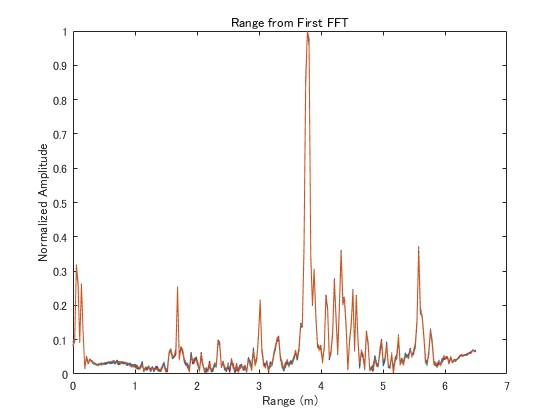
\includegraphics[width=0.8\linewidth]{./img/range_fft_no2division.jpg}
\end{center}
\caption{初めの1フレーム中のTx1→Rx1への信号に対するRange FFT結果}
\end{figure}

図1に送信アンテナ1から受信アンテナ1へのFMCWレーダで得られた信号のうち,初めの1フレームのRange FFTの結果を示しました.期待される信号のピークは,2.5m, 5.0m, 6.0mのあたりに現れることですが,所望のスペクトルを得ることはできませんでした.原因としては,

\begin{itemize}
    \item 最初の1フレームのみを使用した
    \item 複数アンテナを使用していない
    \item 適切な窓関数やCFAR処理を行っていない
    \item 正しいコードではない
\end{itemize}
等が考えられます.何度かコードを修正したり,フレーム数などの条件を変更し,遠藤さんに相談しながら実装・実行を行ってみているのですが,今のところ期待する結果は得られていない状態です.ただし,期待したスペクトルが得られていないだけで,私の使用した初めの1フレームに対するFFT処理(コード)と出力は間違っていない可能性があり,お手本となるものがないため,引き続き試行錯誤の必要があると考えています.また,複数アンテナに対する処理やCFAR処理などの実装も行いたいと思います.

\begin{figure}[H]
\begin{center}
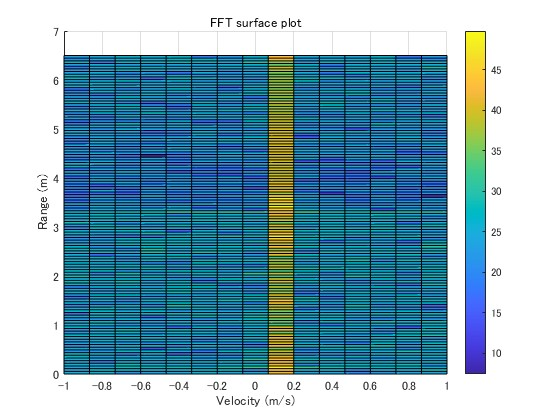
\includegraphics[width=0.8\linewidth]{./img/RDM_shift_division.jpg}
\end{center}
\caption{初めの1フレーム中のTx1→Rx1への信号に対するRange Doppler Map}
\end{figure}

図2にはレンジドップラーマップを示しました.条件は図1と同様です.また,Range軸に対して,期待した出力ではないのも同様となっています.横軸はドップラー速度となっていますが,こちらは軸の値の決め方が分からず,github上のサンプルコード[1]を参考に,仮に-1 m/s ~ 1 m/sとしました.FFTシフトを行い,ゼロ周波数成分をスペクトルの中心に移動しているため,軸の中央の値が0 m/sになると理解しています.
被験者は椅子の上に座って静止しているはずですので,ドップラー速度軸に関しては,ほぼ期待通りの出力と言えると考えられます.

\section{情報工学輪講}
7/30の輪講発表本番では,研究室内発表の2回目で発表した,"Deep generative model with domain adversarial training for predicting arterial blood pressure waveform fromphotoplethysmogram signal"[2]を用いたいと思っております.

情報工学輪講の発表時間は10分だと思いますので,発表用スライドを見直し,短くまとめました.

\section{計画}
\begin{itemize}
    \item 情報工学輪講に向けてスライド仕上げとプレゼン練習をする.
    \item RDMに対し,ハミング窓,ビームフォーミング,CFAR,Angle FFTなどを実装していく.
\end{itemize}

\begin{thebibliography}{}
\item \url{https://github.com/Ram-Godavarthi/Sensor_Fusion_Radar_Target_Generation_and_Detection}
\end{thebibliography}
\end{document}